\section{方法}
本研究で開発するmy\_help2hikiの想定される使用法と設計仕様について記述する.

\subsection{想定している使用法}
設計仕様を決めるために,まず使用法を考える.
想定している使用法は以下の通りである.
\begin{description}
\item 1. my\_helpを利用してメモを作成する.
\item 2. 研究室の各学生のメモを1つの場所に集めるためにサーバに送る.
\item 3. サーバに集めたメモをhikiの形式に変換して,wikiで表示する.
\item 4. 研究室に所属するメンバーが全員のメモを閲覧することで情報を共有する.
\end{description}

\subsection{設計仕様}
3.1で述べた使用法に基づき,設計仕様を考える.
設計仕様は以下の図の通りである.

\begin{figure}[htbp]\begin{center}
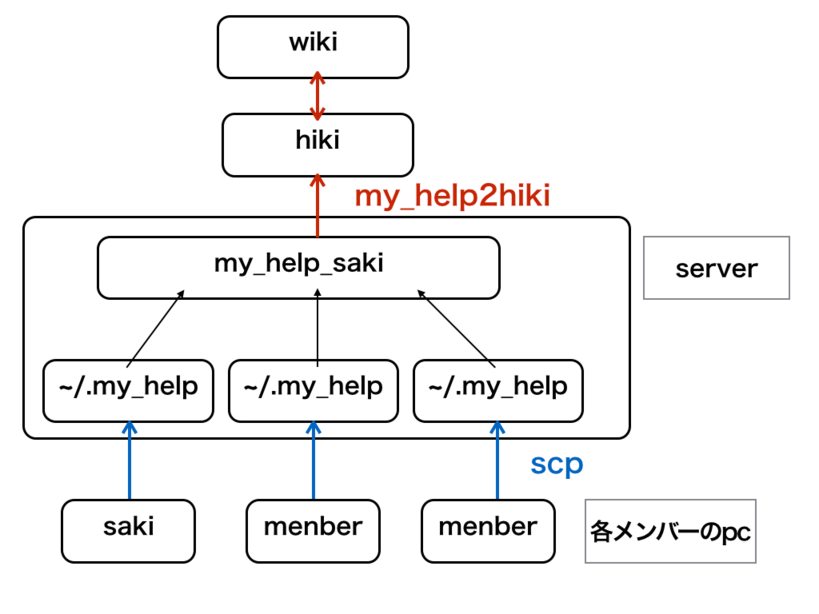
\includegraphics[width=6cm,bb=100 100 600 700]{my_help2hiki_saki.010.png}
\caption{my\_help2hiki}
\label{default}\end{center}\end{figure}

各学生が自分のパソコンでmy\_helpを利用してメモを作成する.
作成したメモは自動的に.my\_helpのディレクトリに保存される.
各自のメモを西谷研究室のサーバのmy\_help\_sakiのディレクトリにscpコマンドを利用してコピーする.
my\_help\_sakiにコピーされたメモをhikiの形式に変換し,wikiで表示する.